../cictikz/src/cictikz/data/tex/cictikz_preamble.tex

% High gate-source voltage: the conduction band at the surface bends
% past the Fermi level - strong inversion.

\definecolor{lblred}{RGB}{160,25,35}
\definecolor{eblue}{RGB}{85,155,235}

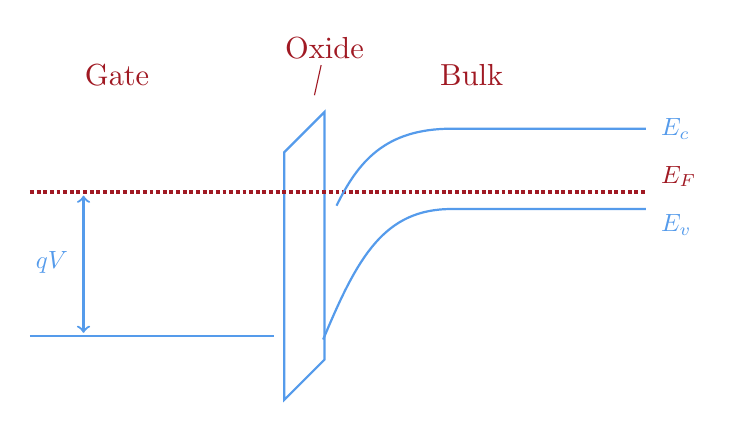
\begin{tikzpicture}[scale=0.85]

  % oxide: vertical interfaces, band edges strongly tilted by the field
  \draw[eblue, thick] (4.1,-1.55) -- (4.1,2.15) -- (4.7,2.75) -- (4.7,-0.95) -- cycle;

  % gate level, far down
  \draw[eblue, thick] (0.3,-0.6) -- (3.95,-0.6);
  \draw[lblred, densely dotted, line width=1.4pt] (0.3,1.55) -- (9.5,1.55);
  \node[lblred, anchor=south west, scale=0.9] at (9.6,1.5) {$E_F$};
  \draw[eblue, thick, <->] (1.1,-0.55) -- (1.1,1.5);
  \node[eblue, anchor=east, scale=0.9] at (1.0,0.5) {$qV$};

  % bulk bands, bending below E_F at the surface
  \draw[eblue, thick]
    (9.5,2.5) -- (6.6,2.5) .. controls (5.6,2.5) and (5.2,2.0) .. (4.88,1.35);
  \node[eblue, anchor=west, scale=0.9] at (9.6,2.5) {$E_c$};
  \draw[eblue, thick]
    (9.5,1.3) -- (6.6,1.3) .. controls (5.6,1.3) and (5.2,0.6) .. (4.68,-0.65);
  \node[eblue, anchor=north west, scale=0.9] at (9.6,1.35) {$E_v$};

  % region labels
  \node[lblred, anchor=center, scale=1.1] at (1.6,3.3) {Gate};
  \node[lblred, anchor=center, scale=1.1] at (4.7,3.7) {Oxide};
  \draw[lblred, thin] (4.65,3.45) -- (4.55,3.0);
  \node[lblred, anchor=center, scale=1.1] at (6.9,3.3) {Bulk};

\end{tikzpicture}
\end{document}
